\chapter{Theoretical Framework}

\section{Forces in Flight}

Fixed-wing aircraft are aerial vehicles whose flight depends on rigid aerodynamic surfaces (airfoils), unlike rotary-wing aircraft that rely on rotating blades to produce thrust and lift.

The fundamental principle of flight is governed by Newton's Second Law, which relates the net force acting on a body to its acceleration:

\begin{equation}
    \vec{F} = m\vec{a}
\end{equation}

where $\vec{F}$ is the resultant force vector, \textit{m} is the aircraft's mass, and $\vec{a}$ is the linear acceleration.

During flight, four main forces act on the aircraft: lift, weight, thrust, and drag. Lift is generated perpendicular to the airflow over the wings and results from a pressure difference between the upper and lower surface of the airfoil, explained by Bernoulli's principle and Newton's Third Law. According to Bernoulli's equation, the sum of static, dynamic pressure, and gravitational potential energy along a streamline is constant:

\begin{equation}
    p + \frac{1}{2} \rho v^2 + \rho g h = constant
\end{equation}

In many aerodynamic cases — like airflow over a wing — the altitude \textit{h}doesn’t change much, so the gravitational term can be neglected, giving the simplified form:

\begin{equation}
    p + \frac{1}{2} \rho v^2 = constant
\end{equation}

However the Bernoulli's principle are impractical for predicting lift in real-world scenarios due to factors like viscosity, turbulence, and three-dimensional flow effects. Therefore, an empirical approach using dimensionless coefficients is often employed. The lift force \textit{L} can be expressed as:

\begin{equation}
    L = C_L \frac{1}{2} \rho v^2 S
\end{equation}

where $C_L$ is the lift coefficient, \textit{$\rho$} is the air density, \textit{v} is the velocity of the aircraft relative to the air, and \textit{S} is the wing area. The lift coefficient $C_L$ is determined experimentally and depends on factors such as the angle of attack, airfoil shape, and Reynolds number.

Drag is the aerodynamic force that opposes the aircraft's motion through the air caused by friction and pressure differences. It can be expressed similarly to lift:

\begin{equation}
    D = C_D \frac{1}{2} \rho v^2 S
\end{equation}

where $C_D$ is the drag coefficient, which also depends on factors like shape, surface roughness, and flow conditions.

Thrust is generated by the aircraft's engines to overcome drag and propel the aircraft forward. The weight ($W = mg$) is the force due to gravity acting downward on the aircraft's mass.

\begin{figure}[H]
    \centering
    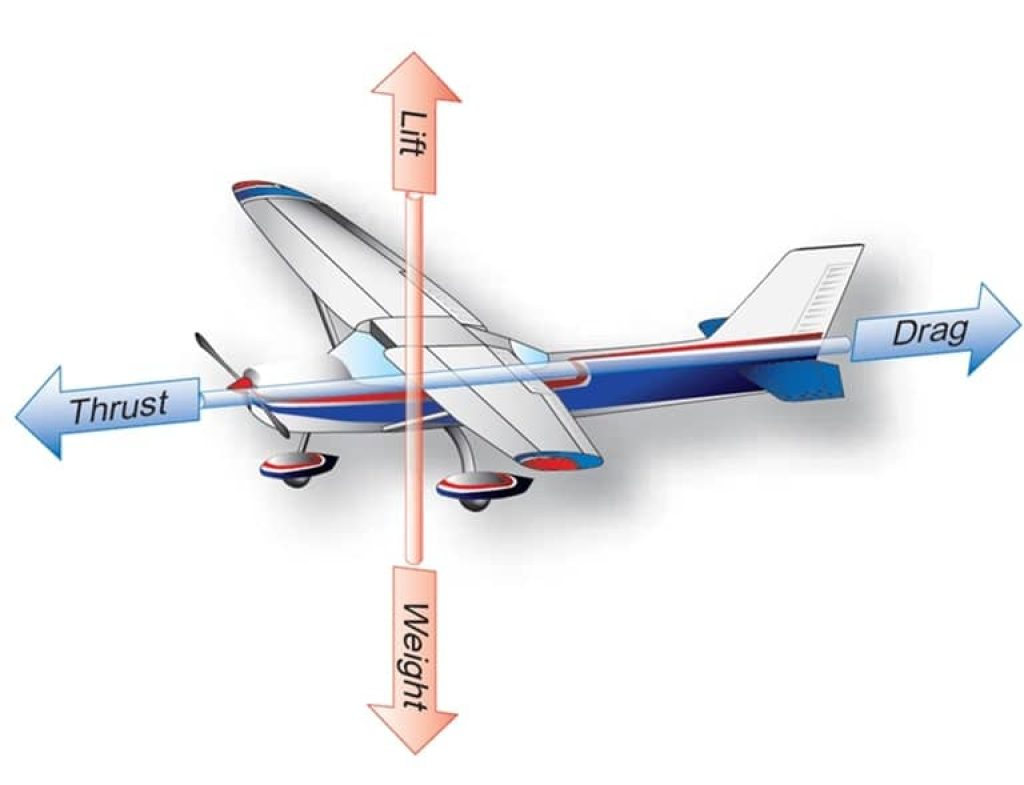
\includegraphics[width=0.8\textwidth]{figures/forces.jpg}
    \caption{Representation of lift and drag forces on a fixed-wing aircraft. \\ Source: StudyFlight (2025). Available at: \url{https://www.studyflight.com/understanding-the-aerodynamic-forces-in-flight/}. Accessed: Oct. 31, 2025.}
\end{figure}


The equilibrium of these forces determines the aircraft's flight conditions, such as steady level flight, climbing, or descending. Control surfaces like ailerons, elevators, and rudders manipulate these forces to change the aircraft's attitude and trajectory.

\section{Flight Dynamics and Control}

% Preciso de um texto que explique a dinâmica de voo e controle de aeronaves, incluindo conceitos como estabilidade, manobrabilidade, e os principais sistemas de controle utilizados em aeronaves. (EM Inglês)

Flight dynamics is the study of the forces and moments that act on an aircraft in flight, and how these affect its motion. Key concepts in flight dynamics include stability and control. Stability refers to the aircraft's ability to return to a steady flight condition after a disturbance. There are three types of stability: static stability, dynamic stability, and maneuverability. Static stability is the initial tendency of the aircraft to return to equilibrium after a disturbance, while dynamic stability refers to the aircraft's response over time. Maneuverability is the aircraft's ability to change its flight path and attitude in response to control inputs.

Aircraft control systems are designed to manage the aircraft's attitude and trajectory. The surfaces can be classified into primary and secondary control surfaces. Primary control surfaces include ailerons, elevators, and rudders, which control roll, pitch, and yaw, respectively. Secondary control surfaces include flaps, slats, and spoilers, which are used to enhance lift or drag during specific flight phases such as takeoff and landing.

\begin{figure}[H]
    \centering
    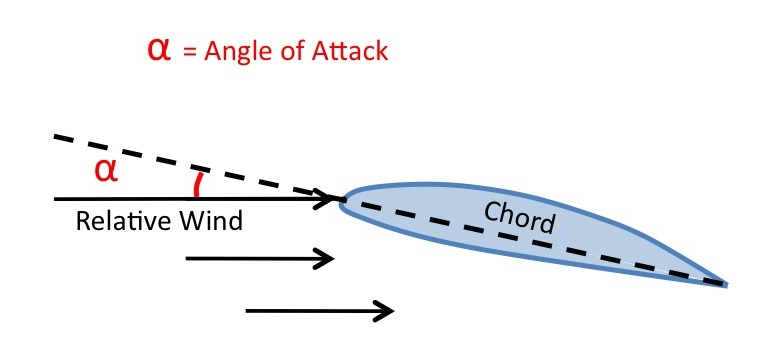
\includegraphics[width=0.6\textwidth]{figures/angle_of_attack.jpg}
    \caption{Illustration of Angle of Attack (AoA) relative to the chord line of an airfoil. \\ Source: NASA (2020). Available at: \url{https://skybrary.aero/articles/angle-attack-aoa}. Accessed: Oct. 31, 2025.}
    \label{fig:angle_of_attack}
\end{figure}

The aircraft's motion can be described in terms of three axes: longitudinal, lateral, and vertical. The longitudinal axis runs from the nose to the tail of the aircraft and is associated with pitch movements, controlled by the elevators. The lateral axis runs from wingtip to wingtip and is associated with roll movements, controlled by the ailerons. The vertical axis runs vertically through the center of gravity and is associated with yaw movements, controlled by the rudder.

The angle of attack (AoA) is a critical parameter in aerodynamics, defined as the angle between the chord line of an airfoil and the oncoming airflow. The chord line is an imaginary straight line connecting the leading and trailing edges of the wing. The AoA significantly influences the lift generated by the wing; as the AoA increases, lift increases up to a certain point known as the critical angle of attack, beyond which the wing may stall due to flow separation.

\begin{figure}[H]
    \centering
    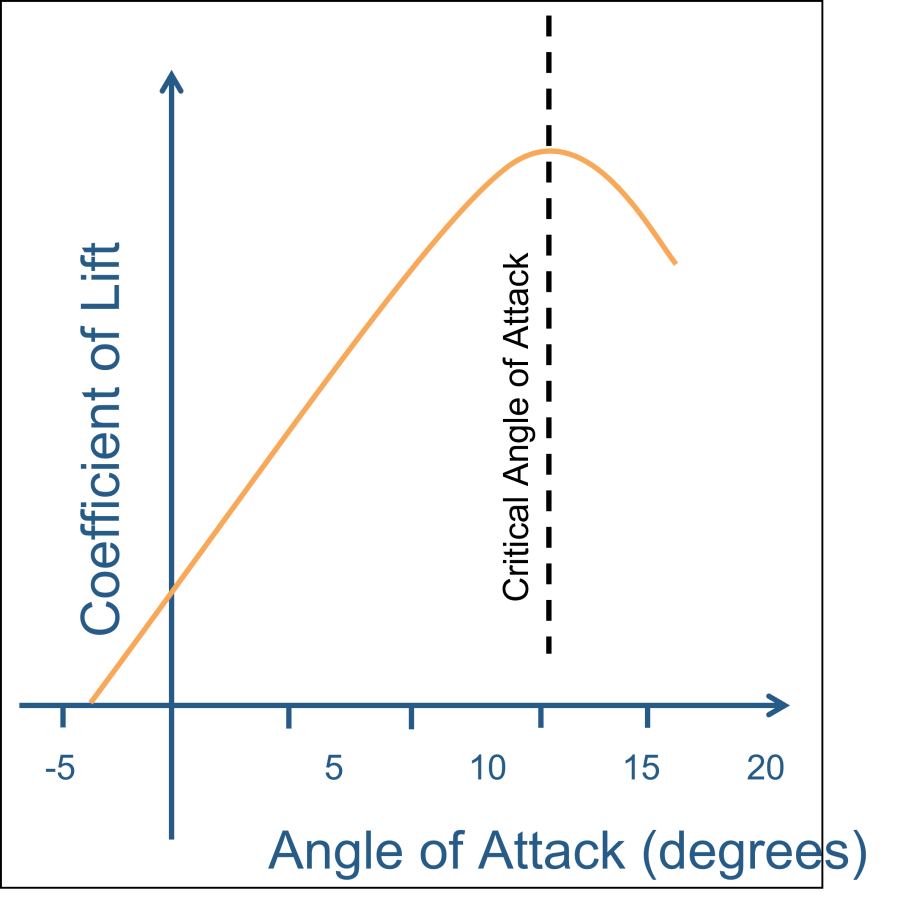
\includegraphics[width=0.7\textwidth]{figures/angle_of_attack_curve.png}
    \caption{Angle of Attack (AoA) curve illustrating the relationship between AoA and lift. \\ Source: NASA (2020). Available at: \url{https://skybrary.aero/articles/angle-attack-aoa}. Accessed: Oct. 31, 2025.}
    \label{fig:angle_of_attack_curve}
\end{figure}

% Explicar como as superfícies de controle (ailerons, rudders, elevators) atuam nesses eixos para controlar a atitude da aeronave fisicamente (com cálculos) (ingles)

The control surfaces of an aircraft play a crucial role in managing its attitude and flight path by acting on the three principal axes: longitudinal, lateral, and vertical. Each control surface is designed to create moments about these axes, allowing the pilot to maneuver the aircraft effectively.

Located on the trailing edges of the wings, ailerons control roll about the longitudinal axis. When the pilot moves the control stick to the left or right, one aileron deflects upward while the other deflects downward. This creates a differential lift on the wings, causing one wing to rise and the other to lower. The rolling moment \( M_{roll} \) generated by the ailerons can be approximated by:

\begin{equation}
    M_{roll} = \frac{1}{2} \rho v^2 S b C_{l_{\delta a}} \delta a
\end{equation}

where \( \rho \) is the air density, \( v \) is the velocity, \( S \) is the wing area, \( b \) is the wingspan, \( C_{l_{\delta a}} \) is the rolling moment coefficient per unit aileron deflection, and \( \delta a \) is the aileron deflection angle.

The horizontal stabilizer also called elevator is located at the tail of the aircraft, elevators control pitch about the lateral axis. When the pilot pulls back on the control stick, the elevators deflect upward, increasing the camber of the horizontal stabilizer and generating a downward force. This causes the nose of the aircraft to rise. The pitching moment \( M_{pitch} \) generated by the elevators can be expressed as:

\begin{equation}
    M_{pitch} = \frac{1}{2} \rho v^2 S c C_{m_{\delta e}} \delta e
\end{equation}

where \( c \) is the mean aerodynamic chord, \( C_{m_{\delta e}} \) is the pitching moment coefficient per unit elevator deflection, and \( \delta e \) is the elevator deflection angle.

The rudders controls yaw about the vertical axis. When the pilot presses the left or right rudder pedal, the rudder deflects to one side, creating a side force that causes the aircraft's nose to yaw in that direction. The yawing moment \( M_{yaw} \) generated by the rudder can be calculated as:

\begin{equation}
    M_{yaw} = \frac{1}{2} \rho v^2 S v_r C_{n_{\delta r}} \delta r
\end{equation}

where \( v_r \) is the distance from the center of gravity to the rudder, \( C_{n_{\delta r}} \) is the yawing moment coefficient per unit rudder deflection, and \( \delta r \) is the rudder deflection angle.

\begin{figure}[H]
    \centering
    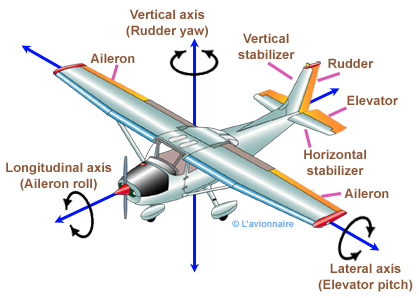
\includegraphics[width=0.8\textwidth]{figures/flight_controls.png}
    \caption{Control surfaces of an aircraft: ailerons, elevators, and rudder. \\ Source: Federal Aviation Administration (2020). Available at: \url{https://www.lavionnaire.fr/AngFlightControl.php}. Accessed: Oct. 31, 2025.}
    \label{fig:control_surfaces}


\section{Related Papers}